\section{ScapeGoat to spot faulty components in a scalable diverse web application}\label{sec:WebStudy}
In this section, we present another application that benefits from the Scapegoat approach.
Although the general goal of spotting components that behave abnormally regarding resource consumption remains the same, with this use case we highlight the possibility of using Scapegoat 
%on a real application 
%and a specific usage of ScapeGoat 
to automatically find buggy components on a scalable modular web application.
The section \ref{MdMS} presents an introduction to the application use case, while the remainder of the section deals with the experimental setup and the results.


\subsection{Use case presentation}\label{MdMS}
We are applying the ScapeGoat approach to check resource consumption contracts on a web application called MdMS.\footnote{https://github.com/maxleiko/mdms-ringojs}
This application offers a web Content Management System based on the Markdown language for editing posts. 
MdMS uses a typical architecture (as shown in Figure \ref{fig:webapp}) for scalable web applications: a load-balancer connected to a set of workers (called MdMS Sosie in the Figure \ref{fig:webapp}), which are themselves connected to a distributed database to retrieve the application specific content.
The worker layer of this application can be duplicated across various machines to support a growing number of clients.
The web application is currently online\footnote{http://cloud.diversify-project.eu/}. 

\begin{figure*}[!bt]
	\centering
	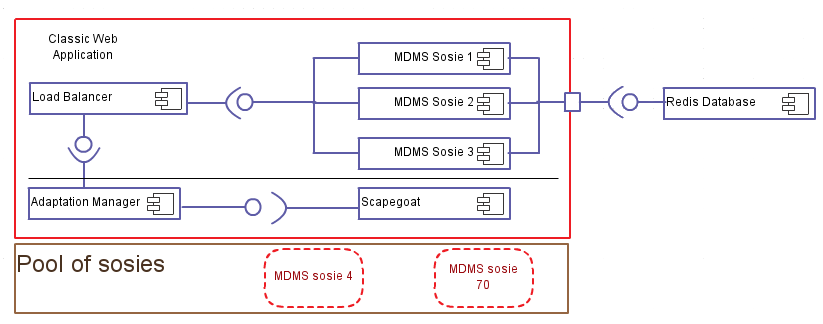
\includegraphics[scale=0.45]{chapter5/figures/webapp}
	\caption{\label{fig:webapp}Architecture of MdMS along with Scapegoat and additional components to adapt th system.}
\end{figure*}

The main characteristic of MdMS is that all workers are not pure clones but diverse implementations of the MdMS server stack~\cite{alliermulti}.
This proactive diversification of MdMS targets safety~\cite{avizienis85} and security~\cite{Forrest97} purposes.
In particular, we have used our recent technique for the automatic synthesis of \textit{sosie} programs~\cite{baudry2014tailored} in order to automatically diversify the workers. 
A \textit{sosie} is a variant of a program that exhibits the same functionality (passes the same test suite) and a diverse computation (different control or data flow). 
\textit{Sosie} synthesis is based on the transformation of the original program through statement deletion, addition or replacement.
%The MdMS application is leveraging this diversified set of workers in order to reach the scalability property while icluding diversity in the software layer to prevent the so-called BOBE (Blow Once, Blow Everywhere) attacks~\cite{alliermulti}.

While the construction of \textit{sosies} focuses on preserving functional correctness, it ignores all the non-functional aspects of the program.
Consequently, a \textit{sosie} offers no guarantee regarding its resource consumption and may contain memory leaks or other overhead on resource consumption that can significantly impact the performance of MdMS.

In this experiment, we use ScapeGoat to monitor the resource consumption of the various \textit{sosies} of the MdMS workers.
This technique enables us to identify \textit{sosies} in a production environment that do not behave according to the resource consumption contracts, allowing the system to remove these workers and use other \textit{sosies}.
Our goal in this experiment is to answer the following research question:

\begin{itemize}
 \item Does ScapeGoat correctly identify the faulty components in a system which includes many variants of the same component?   
\end{itemize}

\subsection{Experimental setup}

We devised this experiment as a scenario where many clients interact with the web application at the same time by adding and removing articles.
The stress produced by these requests increases the resource consumption on the server side which is running on top of Kevoree components.
Figure~\ref{fig:webapp} depicts the server side's configuration.
Since MdMS is a web application developed on top of RingoJS~\footnote{https://github.com/ringo/ringojs}, a JavaScript runtime written in Java, our \textit{sosies} include the RingoJS framework and the application that has been wrapped into Kevoree components.

In this experiment, we deploy many of these components as back-end servers of the web application and we use ScapeGoat to monitor the consumption of each server.
Their contracts regarding resource consumption were built using the mechanism described in section \ref{sec:measurement_metodology} but with the original MdMS worker as a reference component.
The application also contains a component acting as a front-end that evenly distributes the requests among back-end servers.
This load balancer implements a plain round robin policy.
%There is an additional component running on the platform, it is in charge of adapting the system.
%This component reacts to events produced by Scapegoat and modifies the deployed system following the Models@run.time paradigm.

To produce a realistic load on the web server we have recorded a set of standard activities on the MdMS web site using Selenium~\footnote{http://www.seleniumhq.org/}.
We then use the Selenium facilities to replay these activities many times in parallel to provide the required work load on the server.
% of resource consumption, we generate many accesses to the system.
%We use Selenium~\footnote{http://www.seleniumhq.org/} to accomplish this purpose since MdMS is a web application.
Our experimental settings feature 120 clients which are scheduled by a pool of 7 concurrent Selenium workers.
Each client adds 10 articles to the database through the Website GUI, which represents 16 requests per article, for a total of 19200 requests to the MdMS workers sent through the load balancer.
In this experiment, the Selenium workers are executed on the same physical device as the web server, with the same testing platform described in section~\ref{sec:measurement_metodology}.

The experiment is configured as follows.
Using the diversification technique described in~\cite{baudry2014tailored}, we synthesized 20 \textit{sosies} of the MdMS workers.
These \textit{sosies} are used to execute the application with a varying number of back-ends (from 4 to 10).
One particular \textit{sosie} has been modified by hand to ensure that it violates the original component's contract.
We execute all the described components as well as the ScapeGoat components on a single instance of Kevoree.

\subsection{Experimentation results}

Figure~\ref{fig:execution-time-web-app} shows the time required on the server side to reply to all the requests sent by Selenium.
Although the values might look surprisingly high at first, they are in fact the result of a heavily loaded system.
Selenium is actually rendering a couple of web pages for each added article; hence at least 2400 pages are rendered.
Moreover, both clients and servers are sharing resources because they run on the same physical device.
%Another point to highlight is that the time needed to execute all these requests remains stable when no monitoring is used and only changes abruptly when deploying ten \textit{sosies}.
%The execution times remain stable when monitoring is not activated, which is expected because the number of requests does not change between experiments, the load balancer distributes these requests evenly, and we are using the same physical device to execute all back-end servers.
%The stability of the executions when monitoring is not activated is expected because the number of requests does not change between experiments, the load balancer distributes these requests evenly, and we are using the same physical device to execute all back-end servers.
This leads to very stable execution times when monitoring is not activated because the number of requests does not change between experiments, the load balancer distributes these requests evenly, and we are using the same physical device to execute all back-end servers.
%\todo{Please, read below the explanation for: Why the execution time decreases?}
In the \textit{local monitoring} series, the global time to execute decreases until reaching 9 \textit{sosies}.
Although counterintuitive, it is caused by the effect of having \textit{localized monitoring} and \textit{load balancing} at the same time.
For instance, when four \textit{sosies} are used, the monitoring probes are periodically injected into one component out of four, hence roughly a quarter of the requests are handled by a slower \textit{sosie}.
However, with eight components the slow execution path is only taken by around 12.5\% of the requests.
The overhead of \textit{Localized monitoring} when ten \textit{sosies} are deployed increases because the physical machine reaches its limit and begins thrashing.
As a consequence, low-level interactions with the hardware (e.g. cache misses), the operating system and the JVM slow down the execution.
On average, the overhead due to monitoring with both instruction instrumentation and memory instrumentation is 1.59, which is lower than the values shown in section~\ref{sec:OverheadFullMonitoring} for full monitoring despite only one of the instrumentation mechanisms being enabled in those experiments.
The values in this section are better even if we are monitoring both resources because we are using the adaptive approach.
   

\begin{figure*}
 \centering
 \begin{minipage}[t]{0.43\linewidth}
 \centering
 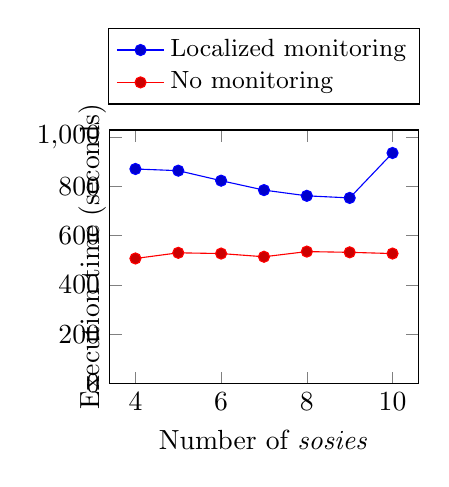
\begin{tikzpicture}
  \begin{axis}[
  	ylabel={Execution time (seconds)},
  	y label style={at={(0.02, 0.5)}},
  	legend style={at={(0.5,1.1)},
  	 	 	anchor=south,legend columns=1, font=\small},
  	ymin=0,
  	every axis legend/.append style={nodes={right}},
  	xlabel={Number of \textit{sosies}},width = 5.5cm,
  	height = 4.8cm]
 
  \addplot+[mark=*] coordinates
  	{(4, 870.375) (5, 863.5) (6, 822.875) (7, 784.625) (8, 761.375) (9, 752.875) (10, 935.3)};

\addplot+[mark=*] coordinates
  	{(4, 507) (5, 530) (6, 527) (7, 514) (8, 535) (9, 532) (10, 527)};
  	
  	\legend{Localized monitoring, No monitoring}
  	
  \end{axis}
  \end{tikzpicture}
  \caption{Time to obtain the reply to all requests.\label{fig:execution-time-web-app}}
  \end{minipage}
  \hspace{0.1\linewidth}
 \begin{minipage}[t]{0.43\linewidth}
 \centering
 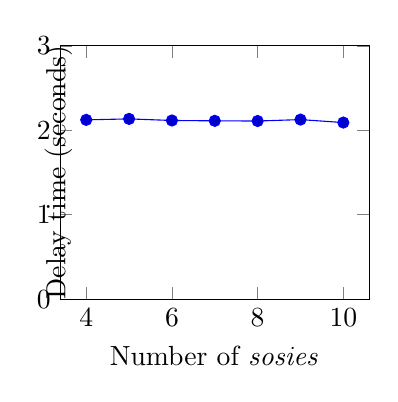
\begin{tikzpicture}
 \begin{axis}[
 	ylabel={Delay time (seconds)},
 	y label style={at={(0.07, 0.5)}}, 	
 	ymin=0,ymax=3,
 	xlabel={Number of \textit{sosies}},width = 5.5cm,
 	height = 4.8cm]

 \addplot+[mark=*] coordinates
 	{(4,2.1235) (5, 2.1348) (6,2.11605) (7,2.1119) (8, 2.1097) (9, 2.12654) (10, 2.09139)};
 	
 \end{axis}
 \end{tikzpicture}
 \caption{Average delay time to detect a faulty \textit{sosie}.\label{fig:delay-time-web-app}}
\end{minipage}

\hspace{1cm}
\end{figure*}


In these experiments, we evaluate the accuracy of the output and its quality in terms of the time needed to find the faulty component.
ScapeGoat always spots the correct \textit{sosie}.
It does so because it is an iterative process that continues until finding the faulty component.
In addition, ScapeGoat does not output false positives during these experiments.
The delay to detect faulty components is shown in Figure~\ref{fig:delay-time-web-app}.
In this case, the values remain close to 2 seconds no matter the number of \textit{sosies} used nor the execution time.
This behavior is consistent with the experiments in section~\ref{sec:evaluation} because we are also using a good heuristic for the use case.
It shows that ScapeGoat can spot faulty components with an acceptable delay in a real application.

\subsection{Discussion of the use case}
%\todo{do something here. JOHANN}
This use case shows that ScapeGoat is able to provide useful information in real applications.
It also highlights how the framework can help select software variants at runtime in the context of software diversity.
Or, more generally, in the field of software oriented architectures where many stakeholders may provide the same services, Scapegoat can help to choose services.
Moreover, this use case leads to a distributed usage of ScapeGoat, where the policies for admission control and resource consumption monitoring can be coordinated among distributed devices.

Finally, in systems where there are many variants of the same component or service, ScapeGoat provides essential information to drive application reconfiguration.
For example, the adaptation component in figure~\ref{fig:webapp} may use Scapegoat's faulty component selection to replace a faulty \textit{sosie} or to modify the scheduling policy in the load balancer.




